\chapter{La trisection d'un angle}\label{c.trisect}

%%%%%%%%%%%%%%%%%%%%%%%%%%%%%%%%%%%%%%%%%%%%%%%%%%%%%%%%%%%%%%%


%%%%%%%%%%%%%%%%%%%%%%%%%%%%%%%%%%%%%%%%%%%%%%%%%%%%%%%%%%%%%%%

Il est impossible de diviser un angle en trois parties égales en utilisant uniquement une règle et un compas. La trisection nécessite la construction de racines cubiques, mais une règle et un compas ne peuvent construire que des longueurs qui sont des expressions construites à partir d'entiers, des quatre opérations  arithmétiques et de racines carrées. Ceci a été démontré par Pierre Wantzel en 1837. Néanmoins, d'innombrables amateurs continuent à rechercher la  trisection d'un angle. Leurs constructions sont des approximations bien qu'ils soient convaincus qu'elles sont correctes. La section~\ref{s.trisect-approx} présente deux de ces constructions, développe des formules pour les angles et montre les erreurs dans les approximations.

Les mathématiciens grecs ont découvert que si d'autres instruments sont autorisés, les angles peuvent être divisés en trois. La section~\ref{s.neusis} explique une construction d'Archimède à l'aide d'un instrument simple appelé \emph{neusis} et la section~\ref{s.neusis-doubling} montre comment dupliquer un cube à l'aide de la \emph{neusis}. La section~\ref{s.q} présente une construction pour la trisection due à Hippias en utilisant un instrument appelé \og quadratrice\fg. Le reste du chapitre contient une démonstration de l'impossibilité de la trisection d'un angle. La section~\ref{s.trisect-constructible} caractérise les nombres constructibles, la section~\ref{s.trisect-poly} relie les nombres constructibles aux racines des polynômes et la section~\ref{s.trisect-impossible} utilise cette théorie pour montrer que la trisection d'un angle et la duplication du cube sont impossibles.

%%%%%%%%%%%%%%%%%%%%%%%%%%%%%%%%%%%%%%%%%%%%%%%%%%%%%%%%

\section{Trisections approximatives}\label{s.trisect-approx}

\subsection{Première trisection approximative}\label{sub.trisect-approx1}

\noindent\textbf{Construction.}
Soit $\theta=\angle AOB$ un angle arbitraire et sans perte de généralité supposons que $A$ et $B$ soient sur un cercle unitaire dont le centre est $O$.  Soit $C$  l'intersection de la bissectrice de $\angle AOB$ avec le cercle unitaire. Soit $D$ le milieu de $\overline{OA}$ et soit $T$ le milieu de $\overline{DC}$. On pose $\phi=\angle DOT$ 
 (fig.~\ref{f.trisect-first-approx-1}).



\begin{figure}[ht]
\centering
\begin{tikzpicture}[scale=.6]
\coordinate (O) at (0,0)
  node[left] {$O$}
  node[above right,xshift=14pt,yshift=16pt] {\sm{\theta/2}}
  node[right,xshift=18pt,yshift=4pt] {\sm{\theta/2}};
\coordinate (A) at (9cm,0);
\node[right] at (A) {$A$};
\coordinate (B) at (60:9);
\node[above] at (B) {$B$};
\draw (A) arc(0:60:9);
\draw (B) -- (O) -- (A);
\coordinate (C) at (30:9);
\node[right] at (C) {$C$};
\draw (O) -- node[above] {$1$} (C);
\coordinate (D) at (4.5,0);
\node[below] at (D) {$D$};
\coordinate (T) at ($(D)!.5!(C)$);
\draw (D) -- node[left] {$a$} (T) -- node[left] {$a$} (C);
\node[right] at (T) {$T$};
\draw (O) -- (T);
\draw (	1,0) arc (0:30:1);
\draw (30:.8) arc (30:60:.8);
\draw (2,0) arc (0:20:2);
\node[above right] at (2.1,0.1) {\sm{\phi}}; 

\draw[<->] (0,-1) -- node[fill=white] {$1/2$} +(4.5,0);
\draw[<->] (4.5,-1) -- node[fill=white] {$1/2$} +(4.5,0);
\end{tikzpicture}
%\includegraphics[width=0.8\textwidth]{Fig2_1}
\caption{Première trisection approximative
 (1).}\label{f.trisect-first-approx-1}
\end{figure}


\begin{theorem}
\[\tan\phi =\frac{2\sin(\theta/2)}{1+2\cos(\theta/2)}\,.\]
\end{theorem}

\begin{proof} La figure~\ref{f.trisect-first-approx-2} est extraite de la figure~\ref{f.trisect-first-approx-1} et contient des annotations supplémentaires.

Soit $\overline{CF}$ la perpendiculaire à $\overline{OA}$ qui coupe $\overline{OA}$ en $F$. Puisque $\overline{OC}=1$, $\overline{CF}=\sin (\theta/2)$ et $\overline{OF}=\cos(\theta/2)$. Soit $\overline{TE}$ la perpendiculaire à $\overline{OA}$ qui coupe $\overline{OA}$ en $E$.

$T$ est le milieu de $\overline{DC}$,  donc $\overline{DT}=\overline{TC}=a$. Mais $\overline{FT}$ est la médiane de l'hypoténuse d'un triangle rectangle, donc $\overline{FT}=a$ et donc $\triangle DTF$ est isocèle. Il s'ensuit que $\overline{TE}$ est à la fois la médiane et la hauteur associée au côté  $\overline{DF}$. D'après la figure, il est facile de voir que 

\begin{figure}[ht]
\centering
\begin{tikzpicture}[scale=.9]
\coordinate (O) at (0,0)
  node[left] {$O$}
  node[right,xshift=24pt,yshift=5pt] {\sm{\theta/2}};
\coordinate (A) at (9cm,0);
\node[right] at (A) {$A$};
\draw (O) -- (A);
\coordinate (C) at (30:9);
\node[right] at (C) {$C$};
\draw (O) -- node[above] {$1$} (C);
\coordinate (D) at (4.5,0);
\node[below] at (D) {$D$};
\coordinate (T) at ($(D)!.5!(C)$);
\draw (D) -- node[left] {$a$} (T) -- node[left] {$a$} (C);
\node[right] at (T) {$T$};
\draw (O) -- (T);
\draw (	1,0) arc (0:30:1);
\draw (2,0) arc (0:20:2);
\node[above right] at (1.9,0.1) {\sm{\phi}}; 

\coordinate (E) at (T |- A);
\draw[thick,dashed] (T) -- node[right] {$h$}
  (E) node[below] {$E$};
\draw[rotate=90] (E) rectangle +(7pt,7pt);

\coordinate (F) at (C |- A);
\draw[thick,dashed] (C) --
  node[right] {$\sin (\theta/2)$} (F) node[below] {$F$};
\draw[rotate=90] (F) rectangle +(7pt,7pt);

\draw[thick,dashed] (T) -- node[right] {$a$} (F);

\draw[<->] ($(O)+(0,-1)$) --
  node[fill=white] {$1/2$} +(4.5,0);
\draw[<->] ($(O)+(0,-1.8)$) --
  node[fill=white] {$\cos (\theta/2)$} ($(F)+(0,-1.8)$);
\draw[<->] ($(D)+(0,-2.6)$) --
  node[fill=white] {$\left(\cos (\theta/2)\!-\! (1/2)\right)$} 
  ($(F)+(0,-2.6)$);
\draw[<->] ($(O)+(0,-3.4)$) --
  node[fill=white] {$(1/2)+(1/2)\left(\cos (\theta/2)\! -\! (1/2)\right)$} 
  ($(E)+(0,-3.4)$);
\end{tikzpicture}
%\includegraphics[width=\textwidth]{Fig2_2}
\caption{Première trisection approximative (2).}\label{f.trisect-first-approx-2}
\end{figure}
\[
\overline{OE}=\frac{1}{2} + \frac{1}{2}\left(\cos \frac{\theta}{2}-\frac{1}{2}\right)\,.
\]
Calculons la longueur $2a=\overline{CD}$ en utilisant le théorème de Pythagore dans  $\triangle DCF$ :
\[
(2a)^2 =  \left(\cos \frac{\theta}{2}-\frac{1}{2}\right)^2+\sin^2\frac{\theta}{2}\,.
\]


La longueur $h=\overline{TE}$ peut être calculée à partir du théorème de Pythagore dans $\triangle DTE$ :
\begin{align*}
a^2 &= h^2 + \left[\frac{1}{2}\left(\cos \frac{\theta}{2}-\frac{1}{2}\right)\right]^2\\
h^2&=\frac{1}{4}\left(\cos \frac{\theta}{2}-\frac{1}{2}\right)^2+\frac{1}{4}\sin^2\frac{\theta}{2}-\left[\frac{1}{2}\left(\cos \frac{\theta}{2}-\frac{1}{2}\right)\right]^2=
\frac{1}{4}\sin^2\frac{\theta}{2}\\
h&=\frac{1}{2}\sin\frac{\theta}{2}\\
\tan\phi &=\frac{h}{\overline{OE}}=\displaystyle\frac{\displaystyle\frac{1}{2}\sin\frac{\theta}{2}}{\displaystyle\frac{1}{2}+\frac{1}{2}\left(\cos \frac{\theta}{2}\! -\! \frac{1}{2}\right)}
=\frac{\displaystyle2\sin\frac{\theta}{2}}{\displaystyle 1+2\cos\frac{\theta}{2}}\,.\qedhere
\end{align*}                  
\end{proof}

C'est une trisection approximative de $\phi=\theta/3$. Pour $\theta=60^\circ$ :
\[
\arctan\left(\frac{2\sin 30^\circ}{1+2\cos 30^\circ}\right)=
\arctan\mbox{0,366}\approx \mbox{20,1}^\circ\approx 20^\circ\,.
\]

Le tableau~\ref{t.trisect-first} montre les erreurs pour une série d'angles aigus. L'erreur est relativement faible pour les petits angles et s'élève à $1\%$ pour  $85^\circ$.

\begin{table}[t]
\caption{Erreurs dans la première trisection approximative.}\label{t.trisect-first}
\[
%
\begin{array}{r@{\hspace{5mm}}r@{\hspace{5mm}}r@{\hspace{5mm}}r@{\hspace{5mm}}r}
\hline
\noalign{\smallskip}
\theta ({}^\circ) & \theta/3 ({}^\circ)& \arctan \phi ({}^\circ) & \mathrm{erreur} ({}^\circ) & \mathrm{erreur (\%)}\\
\noalign{\smallskip}
  5 &    \mbox{1,667} &    \mbox{1,667}  &     \mbox{0,000} &    \mbox{0,004} \\
 10 &    \mbox{3,333} &    \mbox{3,334}  &     \mbox{0,000} &    \mbox{0,014} \\
 15 &    \mbox{5,000} &    \mbox{5,002}  &     \mbox{0,002} &    \mbox{0,032} \\
 20 &    \mbox{6,667} &    \mbox{6,670}  &     \mbox{0,004} &    \mbox{0,057} \\
 25 &    \mbox{8,333} &    \mbox{8,341}  &     \mbox{0,007} &    \mbox{0,088} \\
 30 &   \mbox{10,000} &   \mbox{10,013}  &     \mbox{0,013} &    \mbox{0,128} \\
 35 &   \mbox{11,667} &   \mbox{11,687}  &     \mbox{0,020} &    \mbox{0,174} \\
 40 &   \mbox{13,333} &   \mbox{13,364}  &     \mbox{0,030} &    \mbox{0,228} \\
 45 &   \mbox{15,000} &   \mbox{15,043}  &     \mbox{0,043} &    \mbox{0,289} \\
 50 &   \mbox{16,667} &   \mbox{16,726}  &     \mbox{0,060} &    \mbox{0,358} \\
 55 &   \mbox{18,333} &   \mbox{18,413}  &     \mbox{0,080} &    \mbox{0,435} \\
 60 &   \mbox{20,000} &   \mbox{20,104}  &     \mbox{0,104} &    \mbox{0,520} \\
 65 &   \mbox{21,667} &   \mbox{21,799}  &     \mbox{0,133} &    \mbox{0,612} \\
 70 &   \mbox{23,333} &   \mbox{23,500}  &     \mbox{0,166} &    \mbox{0,713} \\
 75 &   \mbox{25,000} &   \mbox{25,206}  &     \mbox{0,206} &    \mbox{0,823} \\
 80 &   \mbox{26,667} &   \mbox{26,918}  &     \mbox{0,251} &    \mbox{0,941} \\
 85 &   \mbox{28,333} &   \mbox{28,636}  &     \mbox{0,303} &    \mbox{1,068} \\
 \noalign{\smallskip}
 \hline
 \end{array}
\]
\end{table}

\subsection{Deuxième trisection approximative}

\noindent\textbf{Construction.}
Soit $\theta=\angle AOB$ un angle arbitraire et  supposons sans perte de généralité que $A$ et $B$ soient sur un cercle unitaire dont le centre est $O$. Construisons un cercle de rayon $1/3$ avec pour centre $O$ et notons $D$ son intersection avec $\overline{OA}$. Soit $C$ l'intersection de la bissectrice de $\angle AOB$ avec le cercle de rayon $1/3$. Traçons la corde $\overline{CD}$ et les cordes $\overline{AE}=\overline{ET}=\overline{CD}$. Puisque des cordes égales sous-tendent des angles centraux égaux, $\angle TOE=\angle EOA=\phi$ (fig.~\ref{f.trisect-second-approx}).

\begin{figure}[ht]
\centering
\begin{tikzpicture}[scale=.75]
\coordinate (O) at (0,0)
  node[left] {$O$}
  node[above right,xshift=10pt,yshift=12pt] {\sm{\theta/2}};

\coordinate (A) at (9cm,0);
\node[right] at (A) {$A$};
\coordinate (B) at (60:9);
\node[above] at (B) {$B$};
\draw (A) arc(0:60:9);
\draw (B) -- (O) -- (A);
\coordinate (D) at (3,0);
\node[below] at (D) {$D$};
\draw[name path=third] (D) arc(0:60:3);
\coordinate (C) at (30:3);
\node[right] at (C) {$C$};
\draw (O) -- node[above,near end] {\sm{1/3}} (C);
\draw[thick] (D) -- (C);
\coordinate (E) at (10:9);
\node[right] at (E) {$E$};
\draw[thick] (A) -- node[right] {\sm{1/3}} (E);
\coordinate (T) at (20:9);
\node[right] at (T) {$T$};
\draw[thick] (E) -- node[right] {\sm{1/3}} (T);
\draw (O) -- node[above,near end] {$1$} (T);

\draw (	1,0) arc (0:30:1);
\draw (30:.8) arc (30:60:.8);
\draw (4,0) arc (0:20:4);
\node at (4.2,0.35) {$\phi$}; 
\node at (4.1,1.1) {$\phi$}; 

\draw[dashed] (O) --
  node[fill=white,inner sep=0pt,very near start,
       xshift=7pt,yshift=1pt] {\sm{\theta/2}} 
  node[fill=white,near end] {$1$} (E);

\draw[<->] (3,-.8) -- node[fill=white] {$2/3$} +(6,0);
\draw[<->] (0,-.8) -- node[fill=white] {$1/3$} +(3,0);
\end{tikzpicture}
%\includegraphics[width=\textwidth]{Fig2_3}
\caption{Deuxième trisection approximative.}
\label{f.trisect-second-approx}
\end{figure}

\begin{theorem}
\[
\cos\phi=1 - \frac{1}{9}(1-\cos(\theta/2))=1 - \frac{2}{9}\sin^2(\theta/4)\,.
\]
\end{theorem}

\begin{proof} D'après la loi des cosinus dans $\triangle DOC$,
\[
\overline{CD}= \left(\frac{1}{3}\right)^2+\left(\frac{1}{3}\right)^2-2\left(\frac{1}{3}\right)\left(\frac{1}{3}\right)\cos (\theta/2)=\frac{2}{9}(1-\cos(\theta/2))\,.
\]

D'après la loi des cosinus dans  $\triangle EOA$:
\[
\overline{AE} = 1^2+1^2-2\cdot 1\cdot 1\cdot \cos \phi=2(1-\cos \phi)\,.
\]



En égalant les deux expressions pour $\overline{CD}=\overline{AE}$ et en simplifiant, nous obtenons 
\[
\cos \phi = 1 - \frac{1}{9}(1-\cos(\theta/2))\,.
\]
Puisque $\cos 2\alpha= \cos^2 \alpha-\sin^2\alpha=1-2\sin^2\alpha$, et donc $1-\cos 2\alpha=2\sin^2\alpha$, nous avons la formule alternative 
\[
\cos \phi = 1 - \frac{2}{9}\sin^2(\theta/4)\,.\qedhere
\]
\end{proof}

C'est une trisection approximative de $2\phi=\theta/3$. Pour $\theta=60^\circ$,
\[
2\arccos\left(1 - \frac{1}{9}(1-\cos 30^\circ)\right)\approx \mbox{19,8}^\circ\approx 20^\circ\,.
\]

Le tableau~\ref{t.trisect-second-approx} montre les erreurs pour une série d'angles aigus. Cette construction est beaucoup moins précise que celle de la section~\ref{sub.trisect-approx1}.

\begin{table}[t]
\caption{Erreurs dans la deuxième trisection approximative.}\label{t.trisect-second-approx}
\[
%
\begin{array}{r@{\hspace{5mm}}r@{\hspace{5mm}}r@{\hspace{5mm}}r@{\hspace{5mm}}r}
\hline
\noalign{\smallskip}
\theta ({}^\circ) & \theta/3 ({}^\circ)& \arccos 2\phi ({}^\circ) & \mathrm{erreur} ({}^\circ) & \mathrm{erreur (\%)}\\
\noalign{\smallskip}\noalign{\smallskip}
  5 &    \mbox{1,667} &    \mbox{1,667}  &     \mbox{0,000} &    \mbox{0,007} \\
 10 &    \mbox{3,333} &    \mbox{3,332}  &     \mbox{0,001} &    \mbox{0,028} \\
 15 &    \mbox{5,000} &    \mbox{4,997}  &     \mbox{0,003} &    \mbox{0,063} \\
 20 &    \mbox{6,667} &    \mbox{6,659}  &     \mbox{0,008} &    \mbox{0,113} \\
 25 &    \mbox{8,333} &    \mbox{8,319}  &     \mbox{0,015} &    \mbox{0,176} \\
 30 &   \mbox{10,000} &    \mbox{9,975}  &     \mbox{0,025} &    \mbox{0,254} \\
 35 &   \mbox{11,667} &   \mbox{11,626}  &     \mbox{0,040} &    \mbox{0,346} \\
 40 &   \mbox{13,333} &   \mbox{13,273}  &     \mbox{0,060} &    \mbox{0,451} \\
 45 &   \mbox{15,000} &   \mbox{14,914}  &     \mbox{0,086} &    \mbox{0,571} \\
 50 &   \mbox{16,667} &   \mbox{16,549}  &     \mbox{0,118} &    \mbox{0,705} \\
 55 &   \mbox{18,333} &   \mbox{18,177}  &     \mbox{0,156} &    \mbox{0,853} \\
 60 &   \mbox{20,000} &   \mbox{19,797}  &     \mbox{0,203} &    \mbox{1,015} \\
 65 &   \mbox{21,667} &   \mbox{21,408}  &     \mbox{0,258} &    \mbox{1,192} \\
 70 &   \mbox{23,333} &   \mbox{23,011}  &     \mbox{0,322} &    \mbox{1,382} \\
 75 &   \mbox{25,000} &   \mbox{24,603}  &     \mbox{0,397} &    \mbox{1,586} \\
 80 &   \mbox{26,667} &   \mbox{26,185}  &     \mbox{0,481} &    \mbox{1,805} \\
 85 &   \mbox{28,333} &   \mbox{27,756}  &     \mbox{0,577} &    \mbox{2,038} \\
 \noalign{\smallskip}
 \hline
 \end{array}
\]
\end{table}


%%%%%%%%%%%%%%%%%%%%%%%%%%%%%%%%%%%%%%%%%%%%%%%%%%%%%%%%%%%%



\section{Trisection à l'aide d'une \emph{neusis}}\label{s.neusis}


On considère une règle non graduée.  Elle ne peut être utilisée que pour construire une droite entre deux points donnés. Archimède a montré qu'une \emph{neusis}, c'est-à-dire une règle avec deux marques situées à une distance fixe l'une de l'autre, peut être utilisée pour diviser un angle en trois (fig.~\ref{f.neusis}). Nous supposons que la distance entre les marques est  1.

\begin{figure}[htbp]
\centering
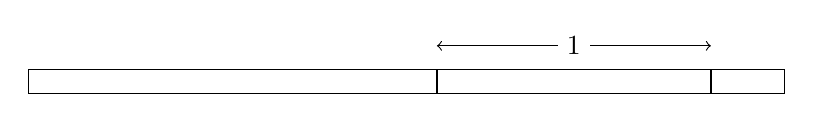
\begin{tikzpicture}[scale=3]
\draw (-1,1.05) rectangle +(3.2,.1);
\draw[thick] (1.89,1.05) -- +(0,.1);
\draw[thick] (.73,1.05) -- +(0,.1);
\draw[<->] (.73,1.25) -- node[fill=white] {$1$} (1.89,1.25);
\end{tikzpicture}
%\includegraphics[width=\textwidth]{Fig2_4}
\caption{Une neusis.}\label{f.neusis}
\end{figure}

\begin{figure}[htbp]
\centering
\begin{tikzpicture}[scale=2.1]
\coordinate (origin) at (0,0) node[below] {$B$} ;
\draw[name path=circle] (origin) circle [radius=1];
\draw (origin) node[above left,xshift=-4pt] {$\alpha$} -- node[fill=white] {$1$} (120:1) coordinate (a) node[below,xshift=-2pt] {$A$} ;
\draw (-1,0) -- (2.5,0);
\path[name path=ad] (a) -- (0,0 -| 2,0) coordinate (d) node[below] {$D$} ;
\path[name intersections={of=circle and ad,by={c,a1}}];
\coordinate (e) at (-1,0);
\vertex{origin};
\node [below,xshift=-4pt] at (c) {$C$};
\node [left] at (e) {$E$};
\node at (1.5,2.5pt) {$\beta$};
\begin{scope}[rotate=-19,yshift=-11.25pt]
\draw (-1,1.05) rectangle +(3.2,.1);
\draw[thick] (1.89,1.05) -- +(0,.1);
\draw[thick] (.76,1.05) -- +(0,.1);
\draw[<->] (.73,1.3) -- node[fill=white] {$1$} (1.89,1.3);
\end{scope}
\end{tikzpicture}
%\includegraphics[width=\textwidth]{Fig2_5}
\caption{La construction par neusis  pour la trisection d'un angle (1).}\label{f.trisect-neusis-1}
\end{figure}

\noindent\textbf{Construction.}
Soit $\alpha=\angle ABE$ un angle arbitraire dans un cercle unitaire de centre $B$, où le rayon du cercle est égal à la distance entre les marques sur la \emph{neusis}. Prolongeons le rayon $\overline{EB}$ au-delà du cercle. Plaçons un bord de la \emph{neusis} sur $A$ et déplaçons-la  jusqu'à ce qu'elle coupe le prolongement de $\overline{EB}$ en $D$ et le cercle en $C$, en utilisant les marques de sorte que la longueur du segment  $\overline{CD}$ soit égale à $1$. Traçons la droite $\overline{AD}$. On note $\angle CDB=\beta$ (fig.~\ref{f.trisect-neusis-1}).

\begin{theorem} $\beta=\alpha/3$.
\end{theorem}
\begin{proof}
Construisons $\overline{BC}$ et désignons les angles et les segments  comme indiqué sur la figure~\ref{f.trisect-neusis-2}.
$\triangle ABC$ et $\triangle BCD$ sont des triangles isocèles : $\overline{AB} = \overline{BC}$ sont des rayons du même cercle et $\overline{BC} = \overline{CD}$ par construction en utilisant la \emph{neusis}. Puisque la somme des angles d'un triangle est égale à $180^\circ$ et que la somme des angles supplémentaires est également égale à $180^\circ$, on a 
\begin{align*}
\epsilon &= 180^\circ - 2\beta\\
\gamma &= 180^\circ - \epsilon = 2\beta\\
\delta &= 180^\circ - 2\gamma = 180^\circ - 4\beta\\
\alpha &= 180^\circ - \delta - \beta=3\beta\,.\qedhere
\end{align*}
\end{proof}

\begin{figure}[htbp]
\centering
\begin{tikzpicture}[scale=2.1]
\coordinate (origin) at (0,0) node[below] {$B$} ;
\draw[name path=circle] (origin) circle [radius=1];
\draw (origin)
  node[above left,xshift=-4pt] {$\alpha$}
  node[above,xshift=4pt,yshift=2pt] {$\delta$}
  node[above right,xshift=30pt,yshift=-2pt] {$\beta$} --
  node[fill=white] {$1$} (120:1)
  coordinate (a) node[above left] {$A$};
\draw (-1,0) -- (2.2,0);
\draw[name path=ad] (a)
  node[below right,xshift=8pt,yshift=-6pt] {$\gamma$} -- 
  (0,0 -| 2,0) coordinate (d)
  node[left,xshift=-24pt,yshift=5pt] {$\beta$}
  node[above right] {$D$};
\path[name intersections={of=circle and ad,by={c,a1}}];
\draw (origin) -- node[fill=white] {$1$}(c) node[above right] {$C$} node[left,xshift=-12pt] {$\gamma$} node[below,xshift=-2pt,yshift=0pt] {$\epsilon$};
\coordinate (e) at (-1,0);
\vertex{origin};
\node [left] at (e) {$E$};
\path (c) -- node[fill=white,near start] {$1$} (d);
\end{tikzpicture}
%\includegraphics[width=0.9\textwidth]{Fig2_6}
\caption{La construction par neusis pour la trisection d'un angle  (2).}\label{f.trisect-neusis-2}
\end{figure}

%%%%%%%%%%%%%%%%%%%%%%%%%%%%%%%%%%%%%%%%%%%%%%%%%%%%%%%%%%%%%


\section{La duplication du cube avec une \emph{neusis}}\label{s.neusis-doubling}

Étant donné un cube $C$, construisons un autre cube ayant deux fois son volume. Si le volume de $C$ est de $V$, ses côtés ont une longueur égale à  $\sqrt[3]{V}$. Les côtés d'un cube dont le volume est double ont une longueur $\sqrt[3]{2 V}=\sqrt[3]{2}\cdot\sqrt[3]{V}$. Donc si nous pouvons construire $\sqrt[3]{2}$, nous pouvons dupliquer le cube.

\smallskip

\noindent\textbf{Construction.}
Construisons le triangle équilatéral $\triangle ABC$ et prolongeons $\overline{CA}$ avec un autre segment de longueur unité jusqu'à $D$. Construisons des demi-droites qui prolongent $\overline{AB}$ et $\overline{DB}$. Plaçons  la \emph{neusis} sur le point $C$ et  déplaçons-la jusqu'à ce qu'une marque de la \emph{neusis} soit placée sur la demi-droite $\overline{AB}$ en $P$ et que l'autre marque soit placée sur la demi-droite  $\overline{DB}$ en $Q$. On note $\overline{CQ}=x$ et $\overline{BP}=y$ (fig.~\ref{f.double-neusis}).

\begin{figure}[htbp]
\centering
\begin{tikzpicture}[scale=.7]
\clip (-.5,-.4) rectangle +(11,6.5);
\coordinate (D) at (0,0) node[left] {$D$};
\draw (D) -- ++(60:6) coordinate (C) node[above] {$C$};
\coordinate (A) at (60:3);
\node[left] at (A) {$A$};
\draw (A) -- ++(3,0) coordinate (B) -- (C);
\node[below right] at (B) {$B$};
\path[name path=DQ] (D) -- ($(D)!1.7!(B)$);
\path[name path=AP] (A) -- ($(A)!3!(B)$);
% 3*(1+\sqrt[3]{2}) = 6.78
\path[name path=CP] (C) circle (6.78cm);
\path[name intersections={of=CP and AP,by={P}}];
\draw[name path=CP] (C) -- (P);
\path[name intersections={of=CP and DQ,by={Q}}];
\node[above] at (Q) {$Q$};
\node[right] at (P) {$P$};
\draw (D) -- (Q);
\draw (B) -- (P);
\path (D) -- node[left] {$1$} (A) -- node[left] {$1$} (C) --
  node[right] {$1$} (B) -- node[below] {$1$} (A);
\path (C) -- node[above] {$x$} (Q) -- node[above] {$1$} (P) -- 
  node[below] {$y$} (B);
\end{tikzpicture}
%\includegraphics[width=0.7\textwidth]{Fig2_7}
\caption{Duplication du cube avec une  neusis.}\label{f.double-neusis}
\end{figure}

\begin{theorem}
$x=\sqrt[3]{2}$.
\end{theorem}

\begin{proof}
Puisque $\triangle ABC$ est équilatéral, $\cos \angle CAP=\cos 60^\circ=\frac{1}{2}$ , et par la loi des cosinus dans $\triangle APC$,
\begin{subequations}
\begin{align}
\overline{CP}&=\overline{AC}^2+\overline{AP}^2-2\cdot \overline{AC}\cdot\overline{AP}\cos 60^\circ\\
(x+1)^2&=1^2+(y+1)^2-2\cdot 1\cdot (y+1)\cdot \frac{1}{2}\\
x^2+2x&=y^2+y\slabel{eq.eq-cube-double}\,.
\end{align}
\end{subequations}

D'après le théorème de Ménélaüs (théorème~\ref{thm.menelaus}),
\[
\displaystyle\frac{\overline{AB}}{\overline{BP}}\cdot
\displaystyle\frac{\overline{PQ}}{\overline{QC}}\cdot
\displaystyle\frac{\overline{CD}}{\overline{DA}}=1\,.
\]



Par conséquent,
\begin{subequations}
\begin{align}
\displaystyle\frac{1}{y}\cdot
\displaystyle\frac{1}{x}\cdot
\displaystyle\frac{2}{1}&=1\\
xy&=2\,.\slabel{eq.menelaus-xy2}
\end{align}
\end{subequations}

En substituant l'équation~\ref{eq.menelaus-xy2} dans l'équation~\ref{eq.eq-cube-double} on obtient
\begin{align*}
x^2+2x&=\frac{4}{x^2}+\frac{2}{x}\\
x^4+2x^3&=4+2x\\
x^3(x+2)&=2(x+2)\\
%x^3&=&2\\
x&=\sqrt[3]{2}\,.\qedhere
\end{align*}
\end{proof}


%%%%%%%%%%%%%%%%%%%%%%%%%%%%%%%%%%%%%%%%%%%%%%%%%%%%%%%%%%%%%
\section{Trisection à l'aide d'une quadratrice}\label{s.q}



Soit $\overline{ABCD}$ un carré. Soit $l_1$ un segment placé initialement en $\overline{DC}$ et soit $l_2$ un segment placé initialement en $\overline{AD}$. Déplaçons $l_1$ à une vitesse constante jusqu'à ce qu'il atteigne $\overline{AB}$ et faisons tourner le segment $l_2$ à une vitesse angulaire constante dans le sens des aiguilles d'une montre autour de $A$ jusqu'à ce qu'il atteigne également $\overline{AB}$. Supposons qu'ils atteignent ensemble $\overline{AB}$. Par exemple, si $l_2$ tourne à $1^\circ$/seconde et que le côté du carré est de $9$ centimètres, $l_1$ doit se déplacer à $0,1$ cm/seconde. La trace de leur point d'intersection $P$ est appelée la \og quadratrice\fg{} (fig.~\ref{f.trisect-quad-curve}). Sa définition est attribuée au mathématicien Hippias.

\vspace{0.4cm}

\begin{minipage}{0.4\textwidth}
\centering   
\begin{tikzpicture}[scale=.4,domain=.03:1.555,samples=100]
\draw (.1,.2)
  node[below left,xshift=-8pt] {$A$} -- 
  (7.8,.2) 
  node[below right] {$B$} -- 
  (8,7.8) 
  node[above right] {$C$} -- 
  (.1,7.8) node[above left,xshift=-8pt] {$D$} -- 
  cycle;
\draw[thick,dashed,name path=arm] (.1,.2) -- node[right,very near end] {$l_2$} (59.6:7.9);
\draw[thick,dashed,name path=horiz] (.1,5) -- node[above,near end] {$l_1$} +(7.8,0);
\path[name intersections={of=arm and horiz,by={A}}];
\node[above left,xshift=-2pt] at (A) {$P$};
\vertex{A};
\draw[thick] plot (4.6*.637*\x,{12.2*.637*\x*cot(\x r)});
\end{tikzpicture}
%\includegraphics[width=\textwidth]{Fig2_8a}
         \captionof{figure}{Une  quadratrice.}\label{f.trisect-quad-curve}
         
     \end{minipage}
     %\hspace{3em}
     \quad 
     \begin{minipage}{0.4\textwidth}
\centering        
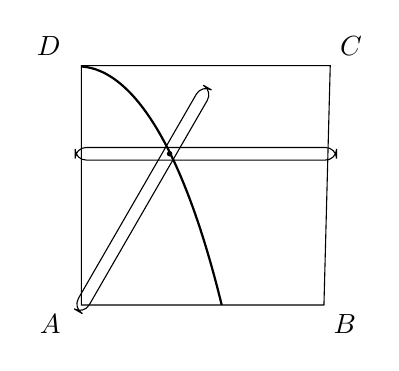
\begin{tikzpicture}[scale=.4,domain=.03:1.555,samples=100]
\draw (.1,.2) node[below left,xshift=-4pt] {$A$} -- (7.8,.2) node[below right] {$B$} -- (8,7.8) node[above right] {$C$} -- (.1,7.8) node[above left,xshift=-4pt] {$D$} -- cycle;
\draw[rounded corners,rotate=60] (0,-.2) rectangle (8.2,.2);
\draw[rounded corners] (-.1,4.8) rectangle (8.2,5.2);
\fill (2.9,5) circle [radius=2.5pt];
\draw[thick] plot (4.6*.637*\x,{12.2*.637*\x*cot(\x r)});
\end{tikzpicture}
%\includegraphics[width=\textwidth]{Fig2_8b}
         \captionof{figure}{Le mécanisme produisant la  quadratrice.}\label{f.trisect-quad-compass}
     \end{minipage}

\vspace{0.4cm}

On peut construire une quadratrice à l'aide d'un mécanisme comme indiqué sur la figure~\ref{f.trisect-quad-compass}. Il se compose de deux règles (non graduées) qui se déplacent comme décrit ci-dessus. Une articulation les contraint à se déplacer ensemble et trace la courbe.

On peut utiliser une quadratrice  pour diviser un angle en trois.

\noindent\textbf{Construction.}
Soit $\angle CDP_1=\alpha$ un angle arbitraire, où $P_1$ est l'intersection de la droite définissant l'angle $\alpha$ par rapport à $\overline{DC}$ et la quadratrice (fig.~\ref{f.trisect-quad-trisect}). Construisons une droite passant par $P_1$ et parallèle à $\overline{DC}$. Notons $E$ son intersection avec $\overline{AD}$. Notons $t$ le segment $\overline{DE}$. Divisons-le en trois (sect.~\ref{s.trisect-constructible}) pour obtenir le point $F$ qui est à une distance $t/3$ de $\overline{DC}$. Soit $P_2$ l'intersection d'une droite qui passe par $F$ et parallèle à $\overline{DC}$ avec la quadratrice. Soit $\theta$ l'angle entre $\overline{DC}$ et $\overline{DP_2}$ (sect.~\ref{f.trisect-quad-trisect}).


\begin{figure}[htbp]
\centering
\begin{tikzpicture}[scale=.8,domain=.03:1.562,samples=100]
\draw (.1,7.8) coordinate (start)
  node[above left] {$D$}
  node[below right,xshift=32pt] {$\theta$} -- 
  (.1,.2) node[below left] {$A$} -- 
  (8,.1)  node[below right] {$B$} -- 
  (8,7.8) node[above right] {$C$} -- 
  cycle;
\draw[name path=curve,thick] plot (4.6*.637*\x,{12.2*.637*\x*cot(\x r)});
% To ensure intersection at node D, path should extend to the upper left of D
\coordinate (twenty-a) at ($(start)+(-35:9)$);
\path[name path=twenty] ($(start)!-.1!(twenty-a)$) -- (twenty-a);
\path[name path=sixty] (start) -- +(-50:11);
\path[name path=xaxis] (.1,.2) -- (8,.1);
\path[name intersections={of=twenty and curve,by={x1,tri}}];
\draw (start) -- (tri);
\node[above right] at (tri) {$P_2$};
\path[name intersections={of=sixty and curve,by={x2,angle}}];
\node[above right] at (angle) {$P_1$};
\draw (start) -- (angle);
\path[name intersections={of=xaxis and curve,by=x}];
\path[name intersections={of=sixty and xaxis,by=sixty-x}];
\draw (start) -- (sixty-x);

\path (tri) -- (tri -| .1,.2) coordinate (t3);
\draw[dashed] (t3) -- +(7.9,0);
\node[left] at (t3) {$F$};
\path (angle) -- (angle -| .1,.2) coordinate (t);
\draw[dashed] (t) -- +(7.9,0);
\node[left] at (t) {$E$};
\draw[<->] (-1.2,7.8) -- node[fill=white] {$t/3$} (-1.2,7.8 |- t3);
\draw[<->] (-.6,7.8) -- node[fill=white] {$t$} (-.6,7.8 |- t);
\draw[<->] (-.6,7.8 |- t) -- node[fill=white] {$1-t$} (-.6,.2);
\draw (3.5,7.8) arc[start angle=0,delta angle=-49,radius=3.5];
\draw (1,7.8) arc[start angle=0,delta angle=-32,radius=1];
\node at (3.3,6) {$\alpha$}; 
\end{tikzpicture}
%\includegraphics[width=\textwidth]{Fig2_9}
\caption{Trisection d'un angle à l'aide d'une quadratrice.}
\label{f.trisect-quad-trisect}
\end{figure}

\begin{theorem}
$\theta = \alpha/3$.
\end{theorem}
\begin{proof}
$E$ a pour ordonnée $1-t$ donc par construction $F$ a pour ordonnée $1-(t/3)$. Puisque la vitesse constante de la droite horizontale est proportionnelle à la vitesse angulaire constante de la droite en rotation, $\theta/\alpha = (t/3)/t$ et $\theta = \alpha/3$.
\end{proof}


\section{Nombres constructibles}\label{s.trisect-constructible}


Soit $l$ un segment  de longueur $1$.

\begin{definition}
Un nombre $a$ est \emph{constructible} si un segment  de longueur $a$ peut être construit à la règle et au  compas à partir de $l$.
\end{definition}

Étant donné le segment $l=\overline{AB}$, construisons une droite contenant $\overline{AB}$ et utilisons le compas pour trouver un point $C$ sur la droite qui est à une distance $1$ de $B$. Alors $\overline{AC}$ a une longueur de $2$ et le nombre $2$ est donc constructible. On peut construire un segment  $\overline{BD}$ de longueur $1$ perpendiculaire à $\overline{AB}$ en $B$. L'hypoténuse du triangle $\triangle ABD$ a une longueur égale à $\sqrt{2}$. Le nombre $\sqrt{2}$ est donc constructible.

\begin{theorem}\label{thm.trisect-constructible}
Un nombre est constructible si et seulement s'il est la valeur d'une expression construite à partir des entiers, des quatre opérations arithmétiques $\{+,-,\times,/\}$ et de l'opération racine carrée $\surd$.
\end{theorem}

\begin{proof} Nous montrons d'abord que les valeurs de ces expressions sont constructibles.


\begin{figure}[htbp]
\centering
\begin{tikzpicture}[scale=.8]
\coordinate (P) at (0,0);
\coordinate (Q) at (5,0);
\coordinate (T) at (3,0);
\coordinate (U) at (7,0);
\vertex{P};
\vertex{Q};
\draw (P) -- (Q);
\node[above] at (P) {$P$};
\node[above left] at (Q) {$Q$};
\node[above left] at (U) {$U$};
\node[above right] at (T) {$T$};
\draw (5,0) -- (8,0);
\draw (5,0) circle[radius=2cm];
\draw (5,0) -- node[left] {$b$} ++(60:2cm);
\coordinate (R) at (9,-1);
\coordinate (S) at ($(9,-1) + (20:2cm)$);
\vertex{R};
\vertex{S};
\draw (R) node[above] {$R$} --
  node[below right] {$b$} (S)
  node[above] {$S$};
\draw[<->] (0,-.5) -- node[fill=white] {$a$} (5,-.5);
\draw[<->] (0,-1) -- node[fill=white] {$a-b$} (3,-1);
\draw[<->] (0,-1.5) -- node[fill=white] {$a+b$} (7,-1.5);
\end{tikzpicture}
%\includegraphics[width=\textwidth]{Fig2_10}
\caption{Construction de l'addition et de la soustraction.}\label{f.trisect-add-subtract}
\end{figure}

\noindent\textbf{Addition et soustraction.}
Étant donné les segments  $\overline{PQ}=a$ et $\overline{RS}=b$, construisons un cercle de centre $Q$ et de rayon $b$ (fig.~\ref{f.trisect-add-subtract}). Prolongeons $\overline{PQ}$ jusqu'à intersecter le cercle en $U$. Alors $\overline{PTQU}$ est un segment avec  $\overline{PT}=a-b$ et $\overline{PU}=a+b$.

\medskip

\noindent\textbf{Multiplication.}
\'Etant donné les triangles semblables dans la figure~\ref{f.trisect-multiplication},
$(1/b)=(a/\overline{OA})$, donc $\overline{OA}=ab$.



\begin{figure}[htbp]
	\centering
        \begin{tikzpicture}[scale=.75]
\draw[name path=horz] (0,0) coordinate (o) -- (7,0);
\node[left] at (o) {$O$};
\coordinate (a) at (6,0);
\node[below]  at (a) {$A$};
\draw (o) -- (30:5.5);
\coordinate (c) at (30:3);
\coordinate (b) at (30:5);
\node[above] at (c) {$C$};
\node[above] at (b) {$B$};
\draw (a) -- (b);
\path[name path=par] (c) -- +($(a)-(b)$);
\path[name intersections={of=par and horz,by=d}];
\node[below] at (d) {$D$};
\draw (c) -- (d);
\draw[<->] (-.4,.5) -- node[fill=white] {$b$} +(30:5.2);
\path (o) -- node[above] {$1$} (c);
\draw[<->] (0,-.8) -- node[fill=white] {$ab$} +(6,0);
\path (o) -- node[below] {$a$} (d);
\end{tikzpicture}
%\includegraphics[width=\textwidth]{Fig2_11a}
         \captionof{figure}{Construction de la multiplication.}\label{f.trisect-multiplication}      
\end{figure}

\medskip

\noindent\textbf{Division.}
\'Etant donné les triangles semblables dans la  figure~\ref{f.trisect-division},
$(1/b)=(\overline{OD}/a)$, donc  $\overline{OD}=(a/b)$.

\begin{figure}[htbp]
	\centering
\centering         
\begin{tikzpicture}[scale=.75]
\draw[name path=horz] (0,0) coordinate (o) -- (7,0);
\node[left] at (o) {$O$};
\coordinate (a) at (6,0);
\node[below]  at (a) {$A$};
\draw (o) -- (30:5.5);
\coordinate (c) at (30:3);
\coordinate (b) at (30:5);
\node[above] at (c) {$C$};
\node[above] at (b) {$B$};
\draw (a) -- (b);
\path[name path=par] (c) -- +($(a)-(b)$);
\path[name intersections={of=par and horz,by=d}];
\node[below] at (d) {$D$};
\draw (c) -- (d);
\draw[<->] (-.4,.5) -- node[fill=white] {$b$} +(30:5.2);
\path (o) -- node[above] {$1$} (c);
\draw[<->] (0,-.8) -- node[fill=white] {$a$} +(6,0);
\path (o) -- node[below] {$a/b$} (d);
\end{tikzpicture}
%\includegraphics[width=\textwidth]{Fig2_11b}
         \captionof{figure}{Construction de la division.}\label{f.trisect-division}
         \end{figure}


\medskip

\noindent\textbf{Racines carrées.}
À partir d'un segment $\overline{BC}=a$, construisons $\overline{AB} =1+a$ et un demi-cercle dont le diamètre est $\overline{AB}$. Construisons une perpendiculaire en  $C$ et considérons  l'intersection $D$ de la perpendiculaire et du cercle (fig.~\ref{f.trisect-square-root}). $\angle ADB$ est un angle droit car il est sous-tendu par un diamètre. \'Etant donné les triangles semblables, $(h/1)=(a/h)$. Donc $h^2=a$ et $h=\sqrt{a}$.

\begin{figure}[htbp]
\centering
\begin{tikzpicture}[scale=1]
\draw[name path=horz] (0,0) coordinate (a) -- (6,0);
\node[left] at (a) {$A$};
\coordinate (b) at (6,0);
\node[below] at (b) {$B$};
\draw[name path=circle] (b) arc(0:180:3);
\path[name path=perp] (2,0) -- +(0,3.2);
\coordinate (c) at (2,0);
\node[below] at (c) {$C$};
\path[name intersections={of=circle and perp,by=d}];
\node[above] at (d) {$D$};
\draw (c) -- node[right] {$h$} (d);
\path (a) -- node[below] {$1$} (c) -- node[below] {$a$} (b);
\draw (c) rectangle +(6pt,6pt);
\draw (a) -- (d) -- (b);
\draw[rotate=-125] (d) rectangle +(6pt,6pt);
\node[above right,xshift=4pt] at (a) {$\alpha$};
\node[above left,xshift=-12pt] at (b) {$90^\circ\!-\!\alpha$};
\node[below right,yshift=-8pt] at (d) {$\alpha$};
\node[below left,xshift=0pt,yshift=-18pt] at (d) {$90^\circ\!-\!\alpha$};
\end{tikzpicture}
%\includegraphics[width=\textwidth]{Fig2_12}
\caption{Construction d'une racine carrée.}
\label{f.trisect-square-root}
\end{figure}

\medskip

Pour démontrer la réciproque du théorème, nous devons déterminer quelles expressions peuvent être construites à la règle et au compas. Il existe trois constructions:\footnote{Pour des raisons de clarté, elles sont illustrées pour des valeurs spécifiques plutôt que pour les équations les plus générales.}

\begin{enumerate}
\item Deux lignes se croisent en un point (fig.~\ref{f.constructible-two-lines}). Les coordonnées de l'intersection peuvent être déduites des équations des deux droites
$y=x$ et $y=4x-2$. Le point d'intersection est $P= (2/3, 2/3)$.

\item Une ligne coupe un cercle en zéro, un ou deux points (fig.~\ref{f.constructible-line-circle}). Les coordonnées des intersections se déduisent des équations de la droite $y=x$ et du cercle $x^2+y^2=4$. Les points d'intersection sont
$P=(\sqrt{2}, \sqrt{2})$ et $Q=(-\sqrt{2}, -\sqrt{2})$.

\item Deux cercles se croisent en zéro, un ou deux points (fig.~\ref{f.constructible-two-circles}). Les coordonnées des intersections se déduisent des équations des deux cercles $(x-1)^2+y^2=4$ et $(x+1)^2+y^2=4$. Les points d'intersection sont $P=(0,\sqrt{2})$ et $Q=(0,-\sqrt{2})$.\qedhere
\end{enumerate}
\end{proof}

\vspace{0.4cm}

\begin{minipage}{0.44\textwidth}
\centering   
\begin{tikzpicture}[scale=.6]
\draw[step=10mm,white!50!black,very thin] (-4,-4) grid (4,4);
\draw[thick] (-4,0) -- (4,0);
\draw[thick] (0,-4) -- (0,4);
\coordinate (O) at (0,0);
\foreach \x in {-3,...,4}
  \node at (\x-.2,-.3) {\sm{\x}};
\foreach \y in {-3,...,-1}
  \node at (-.4,\y-.3) {\sm{\y}};
\foreach \y in {1,...,4}
  \node at (-.3,\y-.3) {\sm{\y}};
\draw[name path=eq1] (-4,-4) -- (4,4);
\draw[name path=eq2] (-.5,-4) -- (1.5,4);
\path[name intersections={of=eq1 and eq2,by={P}}];
\node[right] at (P) {$P$};
\end{tikzpicture}
%\includegraphics[width=\textwidth]{Fig2_13a}
         \captionof{figure}{Le point d'intersection de deux droites.}\label{f.constructible-two-lines}
         
     \end{minipage}
     \quad \ %\hspace{3em}
     \begin{minipage}{0.44\textwidth}
\centering         
\begin{tikzpicture}[scale=.6]
\coordinate (O) at (0,0);
\draw[step=10mm,white!50!black,very thin] (-4,-4) grid (4,4);
\draw[thick] (-4,0) -- (4,0);
\draw[thick] (0,-4) -- (0,4);
\foreach \x in {-3,...,4}
  \node at (\x-.2,-.3) {\sm{\x}};
\foreach \y in {-3,...,-1}
  \node at (-.4,\y-.3) {\sm{\y}};
\foreach \y in {1,...,4}
  \node at (-.3,\y-.3) {\sm{\y}};
\coordinate (A) at (2,0);
\node[draw,circle through=(A),name path=circle] at (0,0) {};
\draw[name path=eq1] (-4,-4) -- (4,4);
\path[name intersections={of=eq1 and circle,by={P,Q}}];
\node[right] at (P) {$P$};
\node[left] at (Q) {$Q$};
\end{tikzpicture}
%\includegraphics[width=\textwidth]{Fig2_13b}
         \captionof{figure}{Les points d'intersection d'une droite et d'un cercle.}\label{f.constructible-line-circle}
     \end{minipage}

\vspace{0.4cm}



\begin{figure}[htbp]
\centering
\begin{tikzpicture}[scale=.66]
\coordinate (O) at (0,0);
\draw[step=10mm,white!50!black,very thin] (-4,-4) grid (4,4);
\draw[thick] (-4,0) -- (4,0);
\draw[thick] (0,-4) -- (0,4);
\foreach \x in {-3,...,4}
  \node at (\x-.2,-.3) {\sm{\x}};
\foreach \y in {-3,...,-1}
  \node at (-.4,\y-.3) {\sm{\y}};
\foreach \y in {1,...,4}
  \node at (-.3,\y-.3) {\sm{\y}};
\coordinate (A) at (3,0);
\node[draw,circle through=(A),name path=circle1] at (1,0) {};
\coordinate (B) at (-3,0);
\node[draw,circle through=(B),name path=circle2] at (-1,0) {};
\path[name intersections={of=circle1 and circle2,by={P,Q}}];
\node[right,xshift=6pt,yshift=-2pt] at (P) {$P$};
\node[right,xshift=6pt,yshift=2pt] at (Q) {$Q$};
\end{tikzpicture}
%\includegraphics[width=0.5\textwidth]{Fig2_14}
\caption{Les points d'intersection de deux cercles.}
\label{f.constructible-two-circles}
\end{figure}



\section{Nombres constructibles comme racines de polynômes}\label{s.trisect-poly}
Pour montrer qu'un nombre n'est pas constructible, nous devons démontrer qu'il ne peut pas être exprimé en utilisant uniquement des nombres entiers et les opérations $\{+,-,\times,/,\surd\}$.

Nous montrerons que les nombres constructibles sont les racines d'une certaine classe de polynômes, puis nous démontrerons que la trisection d'un angle et la duplication d'un cube nécessitent la construction de racines de polynômes qui ne font pas partie de cette classe. Aujourd'hui, ces résultats sont démontrés en utilisant la théorie des corps de l'algèbre abstraite, mais ici nous donnons une démonstration qui utilise les mathématiques élémentaires. La démonstration est basée sur la définition suivante.

\begin{definition}
La profondeur d'une expression construite à partir des entiers et des opérations $\{+,-,\times,/,\surd\}$ est le niveau maximal d'imbrication des racines carrées.
\end{definition}

\begin{example}
Considérons l'expression suivante:
\[
\sqrt{17+3\sqrt{17} - \sqrt{34-2\sqrt{17}}
  -2\sqrt{34+2\sqrt{17}} }\,.
\]
La profondeur est de $3$ car à droite de l'expression nous avons $\sqrt{17}$ qui est imbriqué dans $\sqrt{34+2\sqrt{17}}$, qui à son tour est imbriqué dans  $\sqrt{17+\cdots-\cdots-2\sqrt{34+2\sqrt{17}}}$.
\end{example}

\begin{theorem}
Une expression de profondeur $n$ peut être exprimée sous la forme $a+b\sqrt{c}$ où $a,b,c$ sont des expressions de profondeur au plus $n-1$.
\end{theorem}
\begin{proof}
Des calculs simples montrent que les expressions $(a_1+b_1\sqrt{c})\,\mathit{op}\,(a_2+b_2\sqrt{c})$ pour les opérateurs $\mathit{op}=\{+,-,\times\}$ donnent des expressions $a+b\sqrt{c}$ de profondeur $n-1$. Pour la division, le calcul est un peu plus compliqué:
\begin{align*}
\frac{a_1+b_1\sqrt{c}}{a_2+b_2\sqrt{c}}&=
\frac{(a_1+b_1\sqrt{c})(a_2-b_2\sqrt{c_2})}{(a_2+b_2\sqrt{c})(a_2-b_2\sqrt{c})}\\
&=\frac{a_1a_2-b_1b_2c}{a_2^2-b_2^2c}+\frac{a_2b_1-a_1b_2}{a_2^2-b_2^2c}\sqrt{c}\,,
\end{align*}
qui est de la forme $a+b\sqrt{c}$, où $a$, $b$ et $c$ sont  de profondeur $n-1$.
Enfin, la racine carrée d'une expression de profondeur $n-1$ est une expression de profondeur $n$.
\end{proof}


\begin{theorem}\label{thm.trisect.conjugate}
Soit $p(x)$ un polynôme unitaire de degré 3 à coefficients rationnels:
\[
p(x)=x^3+a_2x^2+a_1x+a_0\,.
\]
Soit $r=a+b\sqrt{c}$ une racine de $p(x)$ de profondeur minimale $n$, où $a,b,c$ sont de profondeur au plus $n-1$. Alors $r'=a-b\sqrt{c}$ est une racine de $p(x)$ et $r\neq r'$.
\end{theorem}



\begin{proof} Calculons $p(r)$ qui est égal à $0$ puisque $r$ est une racine:
\begin{align*}
&(a+b\sqrt{c})^3+a_2(a+b\sqrt{c})^2+a_1(a+b\sqrt{c})+a_0\\
&=(a^3+3a^2b\sqrt{c}+3ab^2c+b^3c\sqrt{c})\\
&\quad+\,a_2(a^2+2ab\sqrt{c}+b^2c) +a_1(a+b\sqrt{c}) +a_0\\
&=(a^3+3ab^2c+a_2a^2+a_2b^2c+a_1a+a_0)\\
&\quad+\,(3a^2b+b^3c+2a_2ab+a_1b)\sqrt{c}\\
&=d+e\sqrt{c}=0\,,
\end{align*}
où $d,e$ sont des expressions de profondeur $n-1$ formées à partir des coefficients rationnels et $a,b,c$. Alors $\sqrt{c}=-d/e$, donc $a+b\sqrt{c}$ peut être exprimé comme une expression de profondeur $n-1$, contredisant l'hypothèse que $a+b\sqrt{c}$ est de profondeur minimale $n$. Puisque $\sqrt{c}\neq 0$  est de profondeur $n$, pour que $d+e\sqrt{c}$ soit nul, il faut que $d=e=0$.

Considérons maintenant $r'=a-b\sqrt{c}$. En examinant le calcul ci-dessus, nous voyons que $p(r')=d-e\sqrt{c}=0+0\cdot\sqrt{c}=0$. Donc $r'$ est aussi une racine de $p$.

Si $r= r'$ alors $0=r-r'=2b\sqrt{c}$, ce qui n'est vrai que si $b=0$. Donc $r$ et $r'$ seraient de profondeur $n-1$, ce qui contredit à nouveau l'hypothèse.
\end{proof}                                

\begin{theorem}
Si un polynôme unitaire de degré 3 à coefficients rationnels 
\[p(x)=x^3+a_2x^2+a_1x+a_0\] n'a pas de racines rationnelles alors aucune de ses racines n'est constructible.
\end{theorem}

\begin{proof} D'après le théorème fondamental d'algèbre (théorème~\ref{thm.fundamental}), $p(x)$ a trois racines $r_1$, $r_2$ et $r_3$. Soit $r_1=a+b\sqrt{c}$ une racine de profondeur minimale $n$. D'après l'hypothèse qu'il n'existe pas de racines rationnelles, on a $n\geq 1$,  donc $b\neq 0$ et $c\neq 0$. D'après le théorème~\ref{thm.trisect.conjugate}, $r_2=a-b\sqrt{c}$ est aussi une racine. Effectuons la multiplication suivante :
\begin{subequations}
\begin{align}
(x-r_1)(x-r_2)(x-r_3)&=x^3 -(r_1+r_2+r_3)x^2\\
&\quad +\, (r_1r_2+r_1r_3+r_2r_3)x + r_1r_2r_3\slabel{eq.viete3}\\
a_2&=-(r_1+r_2+r_3)\\
r_3&=-(a_2+r_1+r_2)\,.
\end{align}
\end{subequations}
Puisque $a_2$ est  rationnel, 
\[r_3=-a_2-(r_1+r_2)=-a_2-2a\,\]
l'est aussi, ce qui 
contredit l'hypothèse.
\end{proof}


\section{Impossibilité des constructions classiques}\label{s.trisect-impossible}

\begin{theorem}\label{thm.trisect.cube-root-irrational}
$\sqrt[3]{2}$ est irrationnel.
\end{theorem}
\begin{proof}
Supposons que $\sqrt[3]{2}$ soit rationnel et égal à $p/q$ où $p$ et $q$ sont des entiers sans facteur commun autre que $\pm 1$. Alors
\begin{eqnarray*}
(p/q)^3&=&(\sqrt[3]{2})^3\\
p^3&=&2q^3\,.
\end{eqnarray*}
Donc $p$ doit être divisible par $2$, disons $p=2r$. Alors 
\begin{eqnarray*}
8r^3&=&2q^3\\
q^3&=&4r^3\,.
\end{eqnarray*}
Donc $q$ est divisible par $2$, ce qui contredit l'hypothèse selon laquelle $p$ et $q$ n'ont pas de facteur commun.
\end{proof}

\begin{theorem}
$x^3-2$ n'ayant pas de racines rationnelles, il est  impossible de dupliquer un cube à la règle et au  compas.
\end{theorem}
\begin{proof} L'une de ses racines est $\sqrt[3]{2}$ qui, selon le théorème~\ref{thm.trisect.cube-root-irrational}, est irrationnelle. Les autres racines sont celles de l'équation du second degré  $x^2+\sqrt[3]{2}x+(\sqrt[3]{2})^2$ obtenue en divisant $x^3-2$ par $x-\sqrt[3]{2}$. Il est facile de vérifier que ses racines ne sont pas rationnelles (en fait, pas même réelles).
\end{proof}


\begin{theorem}
Il est impossible de diviser un angle arbitraire en trois à la règle et au  compas.
\end{theorem}
\begin{proof}
Il suffit de montrer l'impossibilité pour un seul angle. Essayons de diviser $60^\circ$ en trois pour obtenir $20^\circ$. D'après le théorème~\ref{thm.triple-angle},
\begin{align*}
\cos 3\alpha&=4\cos^3\alpha -3\cos\alpha\\
\cos 60^\circ&=4\cos^3 20^\circ -3\cos 20^\circ\,.
\end{align*}
Soient $x=\cos 20^\circ$ et $y=2x$. Puisque $\cos 60^\circ=1/2$, on a 
\begin{align*}
4x^3 -3x-\frac{1}{2} &= 0\\
8x^3-6x-1&=0\\
y^3-3y-1&=0\,.
\end{align*}

Pour démontrer que le polynôme $y^3-3y-1$ n'a pas de racines rationnelles, supposons que $y=a/b$ soit une racine rationnelle avec $a$ et $b$ n'ayant aucun facteur commun autre que $\pm 1$. Alors 
\begin{subequations}
\begin{align}
(a/b)^3-3(a/b)-1&=0\\
a^3-3ab^2&=b^3\\
a(a-3b^2)&=b^3\slabel{eq.trisect1}\\
a^3&=b(b^2+3ab)\slabel{eq.trisect2}\,.
\end{align}
\end{subequations}
D'après  l'équation~\ref{eq.trisect1}, $b$ doit être divisible par $a$, et d'après l'équation~\ref{eq.trisect2}, $a$ doit être divisible par $b$, ce qui n'est possible que si $a=b=\pm 1$ et $a/b=\pm 1$. Le calcul montre que  $y=a/b=1$ et $y=a/b=-1$ ne sont pas des racines du polynôme.
\end{proof}


Une autre façon de démontrer l'impossibilité des constructions est d'utiliser le théorème suivant que nous présentons sans démonstration.

\begin{theorem}\label{thm.factor}
Si un polynôme unitaire  $p(x)=x^n+a_{n-1}x^{n-1}+\cdots+a_0$ avec des coefficients entiers a des racines rationnelles alors il a des racines entières.
\end{theorem}

Pour démontrer l'impossibilité de dupliquer un cube, nous devons démontrer que 
\[
x^3-2=(x-r_2)(x-r_1)(x-r_0)
\]
n'a pas de racines entières. Puisque $r_0r_1r_2=-2$, toutes les racines doivent diviser $2$, donc les seules racines entières possibles sont $\pm 1, \pm 2$. Un calcul rapide montre qu'aucune d'entre elles n'est une racine.

Pour démontrer l'impossibilité de diviser un angle en trois, nous devons montrer que $y^3-3y-1$ n'a pas de racines entières. Une racine entière doit diviser $-1$ mais ni $1$ ni $-1$ ne sont des racines.

\subsection*{Quelle est la surprise ?}

Underwood Dudley a fait une étude approfondie de ce qu'il appelle les \og grincheux\fg{} qui perdent des années de leur vie à essayer de diviser les angles en trois à la règle et au compas. Non seulement ils s'illusionnent en pensant que c'est possible, mais, pire encore, ils pensent qu'une solution serait importante. Bien sûr, une solution n'aurait aucune utilité pratique, puisque des outils tels que la \emph{neusis} et la quadratrice peuvent résoudre le problème exactement. Le nombre de ces constructions est surprenant, d'autant plus que beaucoup d'entre elles sont astucieuses et permettent d'obtenir de bonnes approximations. Le calcul des formules associées à ces constructions est un excellent exercice de trigonométrie.

Il est également surprenant que les preuves de l'impossibilité de ces constructions géométriques soient purement algébriques et utilisent les propriétés des racines des polynômes.

\subsection*{Sources}

Wikipédia \cite{wiki:tri, wiki:neu, wiki:quad} est une bonne source pour les constructions de ce chapitre.
Les deux trisections approximatives proviennent de \cite [p.
~67--68, 95--96]{dudley-budget}. Le deuxième exemple est attribué au célèbre philosophe Thomas Hobbes. Tant \cite[p.~48--49]{martin} que \cite[p.~6--7]{dudley-budget} traitent de la trisection à l'aide d'une quadratrice.
La duplication du cube à l'aide d'une \emph{neusis} est reprise de \cite{dorrie2}.

Un traitement rigoureux de la constructibilité peut être trouvé dans les manuels d'algèbre abstraite tels que \cite{fraleigh}, qui contient une démonstration générale de la réciproque du théorème~\ref{thm.trisect-constructible} dans la section~32.
Le théorème~\ref{thm.factor} est 
 le théorème~23.11 de \cite{fraleigh}.
Une présentation relativement accessible de la démonstration de Wantzel se trouve dans \cite{suzuki}. Notre présentation de la constructibilité est basée sur les présentations de \cite[chap.~III]{courant} et \cite{laugwitz}.
